%!TEX root = ../DigSig2.tex
\section{DFT/FFT Algorithms\buch{Chapter 9}}

\subsection{Basics}

\begin{description}
	\item[DTFT] Discrete-time Fourier transform \\
		Discrete time-domain, continuous frequency-domain.
	\item[DFT] Discrete Fourier transform \\
		Both time-domain and frequency-domain are discrete.
	\item[FFT] Fast Fourier transform \\
		A fast implementation of the DFT.
\end{description}

\subsection{Frequency Resolution and Windowing\buchSeite{464-472}}

Given an infinite sampled sequence $x(nT)$, to calculate its spectrum a finite
number of samples $L$ has to be cut out using a window function $w(n)$.
At the sampling time interval $T = 1/f_s$, the duration of the data record
is $T_L = LT$. \\

The finite signal $x_L$ is achieved by
\begin{equation*}
	x_L(n) = x(n) w(n)
\end{equation*}
using one of the below defined window functions. \\

\paragraph{Rectangular Window}
	\begin{equation*}
		w(n) = \begin{cases}
			1, & \text{if} \: 0 \leq n \leq L-1 \\
			0, & \text{otherwise}
		\end{cases}
	\end{equation*}

\paragraph{Hamming Window}
	\begin{equation*}
		w(n) = \begin{cases}
			0.54-0.46 \cos\left(\frac{2 \pi n}{L-1}\right), & \text{if} \: 0 \leq n \leq L-1 \\
			0, & \text{otherwise}
		\end{cases}
	\end{equation*}

The constant $c$, which depends on the window, is introduced. For the
\emph{rectangular} window, $c=1$, for the \emph{Hamming} window, $c=2$.
$c$ is always greater than one. \\

The mainlobe width of a given window is defined as
\begin{equation*}
	\Delta\omega_w = c \cdot \frac{2 \pi}{L} \qquad \text{or} \qquad \Delta f_w = c \cdot \frac{1}{T_L}
\end{equation*}

The relative sidelobe level is
\begin{equation*}
	R = 20 \log_{10} \left| \frac{W(\omega)}{W(0)} \right|
\end{equation*}
at $\omega = $ position of the first sidelobe. ($\omega=3\pi/L$ for the
rectangular window). This leads to $R = -13.46 dB$ for the rectangular
and $R = -40 dB$ for the Hamming window. \\

The frequency resolution, i.e. the condition that two sinusoids appear as
two distinct ones is then
\begin{equation*}
	 \Delta\omega \geq \Delta\omega_w = c \cdot \frac{2 \pi}{L}\qquad \text{or} \qquad \Delta f \geq \Delta f_w = c \cdot \frac{f_s}{L}
\end{equation*}

For a given frequency resolution, the window length is therefore
\begin{equation*}
	L \geq c \cdot \frac{f_s}{\Delta f} = c \cdot \frac{2 \pi}{\Delta \omega}
\end{equation*}

\subsection{DTFT Computation\buchSeite{475-482}}

\subsubsection{DTFT at a Single Frequency\buchSeite{475-477}}
\begin{align*}
X(\omega) & = \sum_{n=0}^{L-1}x(n)e^{-j\omega n}
 	  = \left.\sum_{n=0}^{L-1}x(n)z^{-n}\right|_{z=e^{j\omega}} \\
	& = \left. X(z)\right|_{z=e^{j\omega}}
\end{align*}

This polynomial can be evaluated using \emph{Hörner's rule}:
\begin{lstlisting}[mathescape]
for $\text{each complex}$ z do:
	X = 0
	for n = L-1 down to n = 0 do:
	  X = x$_n$ + z$^{-1}$X
\end{lstlisting}
for example, let $L=4$:
\begin{align*}
	X &= 0 \\
	X &= x_3+z^{-1}X = && x_3 \\
	X &= x_2+z^{-1}X = && x_2+z^{-1}x_3 \\
	X &= x_1+z^{-1}X = && x_1+z^{-1}x_2+z^{-2}x_3 \\
	X &= x_0+z^{-1}X = && x_0+z^{-1}x_1+z^{-2}x_2+z^{-3}x_3 = X(z) \\
\end{align*}

\subsubsection{DFT\buchSeite{479-481}}
The $N$-point DFT of a length-$L$ signal is defined as the DTFT evaluated
at $N$ equally spaced frequencies over the full Nyquist interval,
$0 \leq \omega \leq 2 \pi$. These frequencies are
\begin{equation*}
	\omega_k = \frac{2 \pi k}{N}\:, \qquad f_k = \frac{k f_s}{N} \:,\qquad k=0,1,\ldots,N-1
\end{equation*}

Thus, the DFT is
\begin{equation*}
	X(\omega_k) = \sum\limits_{n=0}^{L-1} x(n) e^{-j\omega_kn} = \sum\limits_{n=0}^{L-1} x(n)z_k^{-n}
\end{equation*}
where $z_k$ are the $N$ths roots of unity
\begin{equation*}
	z_k = e^{j\omega_k} = e^{2\pi j k / N}
\end{equation*}
which leads to
\begin{equation*}
	\omega_{k+N} = \omega_k + 2 \pi \qquad \text{and} \qquad X(k+N) = X(k)
\end{equation*}

The bin width is then
\begin{equation*}
	\Delta\omega_{bin}=\frac{2\pi}{N} \qquad \text{or} \qquad \Delta f_{bin}=\frac{f_s}{N}
\end{equation*}


\subsubsection{Zero Padding\buchSeite{481}}
Note that $L$ is the number of time moments and $N$ is the number of
frequency points. Mostly $L=N$ is used. For $L<N$, zero padding can be used
to make the time sequence longer. For $L>N$, a modulo-N wrapping can be
used to make the time sequence shorter. \\

Adding any number of zeros to the end of a signal does \emph{not} change its DTFT!
\begin{align*}
	\mathbf{x} &= [x_0,x_1,\ldots,x_{L-1}] \\
	\mathbf{x}_D &= [x_0,x_1,\ldots,x_{L-1},\underbrace{0,0,\ldots,0}_{D \text{ zeros}}] \\
	X_D(\omega_k) &= X(\omega_k)
\end{align*}

Adding zeros in front adds a linear phase term.
\begin{align*}
	\mathbf{x} &= [x_0,x_1,\ldots,x_{L-1}] \\
	\mathbf{x}_D &= [\underbrace{0,0,\ldots,0}_{D \text{ zeros}},x_0,x_1,\ldots,x_{L-1}] \\
	X_D(\omega_k) &= e^{-j \omega_k D} X(\omega_k)
\end{align*}

\subsection{Physical vs Computational Resolution\buchSeite{482-485}}

\emph{Physical} frequency resolution is defined as
\begin{equation*}
	\Delta f_w = c \cdot \frac{f_s}{L}
\end{equation*}
whereas the \emph{computational} frequency resolution is
\begin{equation*}
	\Delta f_{\text{bin}} = \frac{f_s}{N}
\end{equation*}

The DFT index $k$ is proportional to the frequency $f$ via
\begin{equation*}
	k = N\:\frac{f}{f_s}\:, \qquad 0\leq k \leq N \text{ and } 0 \leq f \leq f_s
\end{equation*}

Ideally, each frequency $f_0$ in the original signal coincides with one
of the $N$ DFT frequencies $f_s k / N$. This is so if $k_0$ is an integer.
\begin{equation*}
	k_0 = N \frac{f_0}{f_s}
\end{equation*}
Usually, this is not the case and the DFT will miss the peak. If $N$ is large
enough, the \emph{rounding error} $= f_s / 2N$ will stay small enough. \\

The \emph{biasing error}, on the other hand, can only be decreased by
increasing the data length $L$, because the DFT is only a sampled version
of the DTFT.


\subsection{Matrix Form of DFT\buchSeite{486-488}}
The DFT can be defined as a linear matrix transformation

\begin{equation*}
	\mathbf{X} = \DFT(\mathbf{x}) = A \mathbf{x}
\end{equation*}

The matrix $A$ for a $N$-point DFT can be built using the so-called
\emph{twiddle factor}.
\begin{equation*}
	W_N = e^{-2 \pi j / N}
\end{equation*}

The matrix elements $A_{kn}$ are found using the definition
\begin{equation*}
	A_{kn} = W_N^{kn}
\end{equation*}

The powers of the twiddle factors are the $N$-th roots of unity:
\begin{center}
	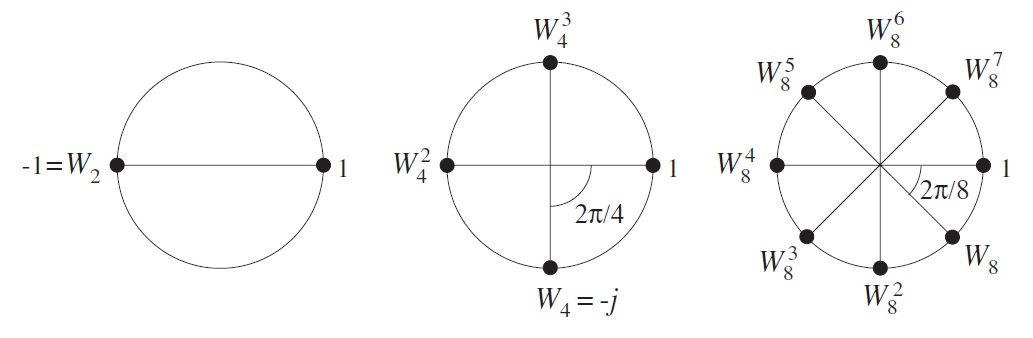
\includegraphics[width=0.9\linewidth]{images/DFT_FFT_WN.jpg}
\end{center}

Some examples of twiddle factors and DFT matrices (see appendix
\ref{app:DFT} for more examples):

\begin{align*}
	W_2 &= e^{-2\pi j / 2} = -1 \\
	W_4 &= e^{-2\pi j / 4} = \cos(\pi/2) - j\sin(\pi/2) = -j \\
	W_8 &= e^{-2\pi j / 8} = \cos(\pi/4) - j\sin(\pi/4) = \frac{1-j}{\sqrt{2}}
\end{align*}

\begin{align*}
	A_2 &=
		\begin{bmatrix}
			1& 1 \\
			1& W_2 \\
		\end{bmatrix}
		&&=
		\begin{bmatrix}
			1& 1 \\
			1& -1 \\
		\end{bmatrix}	 \\
	A_4 &=
		\begin{bmatrix}
			1& 1& 1& 1 \\
			1& W_4& W_4^2& W_4^3 \\
			1& W_4^2& W_4^4& W_4^6 \\
			1& W_4^3& W_4^6& W_4^9 \\
		\end{bmatrix}
		&&=
		\begin{bmatrix}
			1& 1& 1& 1 \\
			1& -j& -1& j \\
			1& -1& 1& -1 \\
			1& j& -1& -j \\
		\end{bmatrix}
\end{align*}

\subsection{Modulo-N reduction\buchSeite{489-496}}
Modulo-N reduction is applied if $L>N$.  The input signal is divided into
non-overlapping blocks of length $N$ and added up.

\begin{center}
	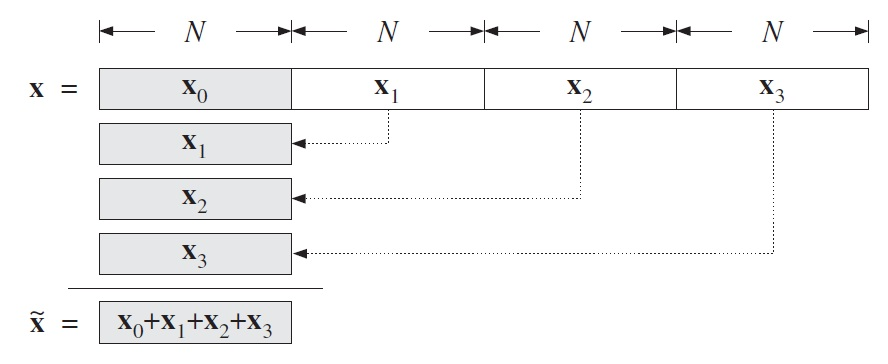
\includegraphics[width=0.8\linewidth]{images/DFT_FFT_ModuloN.jpg}
\end{center}

\begin{equation*}
	\tilde{\mathbf{x}} = \mathbf{x}_0 + \mathbf{x}_1 + \mathbf{x}_2 + \mathbf{x}_3
		\quad \text{or} \quad
	\tilde{x}(n) = \sum\limits_{m=0}^{\infty} x(mN + n)
\end{equation*}

The proof that $\mathbf{X} = \tilde{\mathbf{X}}$ is that

\begin{align*}
	\mathbf{X} &= Ax = [\tilde{A},\tilde{A},\ldots,\tilde{A}]
		\begin{bmatrix}
			\mathbf{x}_0 \\ \mathbf{x}_1 \\ \vdots \\ \mathbf{x}_n
		\end{bmatrix}
		= \tilde{A} \mathbf{x}_0 + \tilde{A} \mathbf{x}_0 + \ldots \\
	&= \tilde{A}(\mathbf{x}_0 + \mathbf{x}_1 + \ldots + \mathbf{x}_n) = \tilde{A}\tilde{\mathbf{x}} = \tilde{\mathbf{X}}
\end{align*}

Similarly, a Matrix $A$ can be created to transform e.g. a length-8 time signal
into a 4-point DFT:
\begin{equation*}
	A = \left[\tilde{A},\tilde{A}\right] = \left[ \begin{array}{cccc|cccc}
		1 & 1 & 1 & 1 & 1 & 1 & 1 & 1 \\
		1& W_4& W_4^2& W_4^3 & 1& W_4& W_4^2& W_4^3 \\
		1& W_4^2& W_4^4& W_4^6 & 1& W_4^2& W_4^4& W_4^6 \\
		1& W_4^3& W_4^6& W_4^9 & 1& W_4^3& W_4^6& W_4^9 \\
	\end{array} \right]
\end{equation*}

\subsection{Inverse DFT\buchSeite{496-499}}
The problem of inverting an $N$-point DFT is that all signals $\mathbf{x}$
with the same modulo-$N$ reduction $\tilde{\mathbf{x}}$ have the same
$N$-point DFT.

\begin{equation*}
	\mathbf{X} = A \mathbf{x} = \tilde{A} \tilde{\mathbf{x}}
\end{equation*}

which means that only the modulo-$N$ reduction of the input signal $\mathbf{x}$
can be reconstructed. Thus
\begin{align*}
	\tilde{\mathbf{x}} = \mathbf{x} \qquad & \text{if} \quad N \geq L \\
	\tilde{\mathbf{x}} \neq \mathbf{x} \qquad & \text{if} \quad N < L
\end{align*}

The inverse DFT is thus defined as
\begin{equation*}
	\tilde{\mathbf{x}} = \text{IDFT}(\mathbf{X}) = \tilde{A}^{-1} \mathbf{X}
\end{equation*}

As $\frac{1}{N} \tilde{A} \tilde{A^*} = I_N$, the inverse of the matrix
$\tilde{A}$ can be obtained by $\tilde{A}^{-1} = \frac{1}{N} \tilde{A}^*$,
which leads to the definition
\begin{equation*}
	\tilde{\mathbf{x}} = \text{IDFT}(\mathbf{X}) = \frac{1}{N} \tilde{A}^* \mathbf{X} = \frac{1}{N}\left[ \DFT(\mathbf{X}^*) \right] ^*
\end{equation*}

\subsection{FFT\buchSeite{504-515}}
The fast Fourier transform (FFT) is a fast implementation of the DFT.
Not an approximation! \\

The FFT calculates the DFT using a divide-and-conquer strategy. It is based
dividing the dimensions of the DFT in half until it becomes one. Hence
the dimension $N$ of the FFT is usually a power of 2: $N = 2^B$. \\

The computational cost can be reduced from $N^2$ for the DFT to $\frac{1}{2} N \log_2 (N)$ for the FFT. \\

A length-$N$ sequence $x(n)$ can be divided into two length-$(N/2)$ subsequences:
\begin{align*}
	\begin{array}{ll}
		g(n) &= x(2n) \\
		h(n) &= x(2n+1)
	\end{array}
	\:,\qquad n = 0,1,\ldots \frac{N}{2}-1
\end{align*}
with their corresponding DFTs
\begin{align*}
	\begin{array}{ll}
		G(k) &= \sum\limits_{n=0}^{N/2-1} W_{N/2}^{kn} \: g(n) \\
		H(k) &= \sum\limits_{n=0}^{N/2-1} W_{N/2}^{kn} \: h(n)
	\end{array}
	\:,\qquad k=0,1,\ldots \frac{N}{2}-1
\end{align*}

The DFT of the original sequence $x(n)$ is obtained by
\begin{equation*}
	X(k) = G(k) + W_N^k H(k) \:,\qquad k=0,1,\ldots,N-1
\end{equation*}

The \emph{butterfly merging} equations follow from the periodicity properties
of the DFT and the fact that the twiddling factor $W_N^{N/2} = -1$:
\begin{align*}
	\begin{array}{rl}
		X(k) = & G(k) + W_N^k H(k) \\
		X(k+N/2) = & G(k) - W_n^k H(k)
	\end{array} \\
	\text{with}\qquad k=0,1,\ldots,\frac{N}{2}-1
\end{align*}

or more easily shown in a vector form:
\begin{align*}
	\begin{bmatrix}	X_0 \\ X_1 \\ \vdots \\ X_{N/2-1} \end{bmatrix} &=
	\begin{bmatrix}	G_0 \\ G_1 \\ \vdots \\ G_{N/2-1} \end{bmatrix} +
	\begin{bmatrix}	H_0 \\ H_1 \\ \vdots \\ H_{N/2-1} \end{bmatrix} \times
	\begin{bmatrix}	W^0_N \\ W^1_N \\ \vdots \\ W^{N/2-1}_N \end{bmatrix}
	\\
	\begin{bmatrix}	X_{N/2} \\ X_{N/2+1} \\ \vdots \\ X_{N-1} \end{bmatrix} &=
	\begin{bmatrix}	G_0 \\ G_1 \\ \vdots \\ G_{N/2-1} \end{bmatrix} -
	\begin{bmatrix}	H_0 \\ H_1 \\ \vdots \\ H_{N/2-1} \end{bmatrix} \times
	\begin{bmatrix}	W^0_N \\ W^1_N \\ \vdots \\ W^{N/2-1}_N \end{bmatrix}
\end{align*}

or even graphically:
\begin{center}
	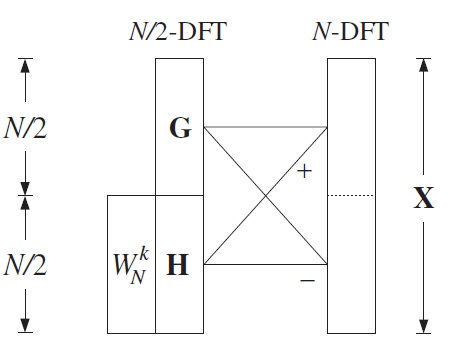
\includegraphics[width=0.5\linewidth]{images/DFT_FFT_butterfly.jpg}
\end{center}

The FFT can easily be summarized by:
\begin{center}
	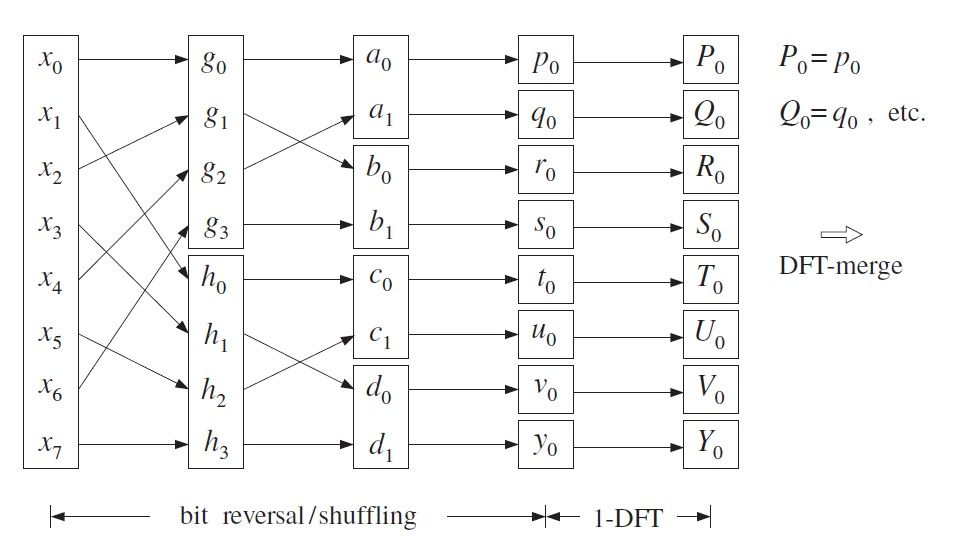
\includegraphics[width=\linewidth]{images/DFT_FFT_step1.jpg}
	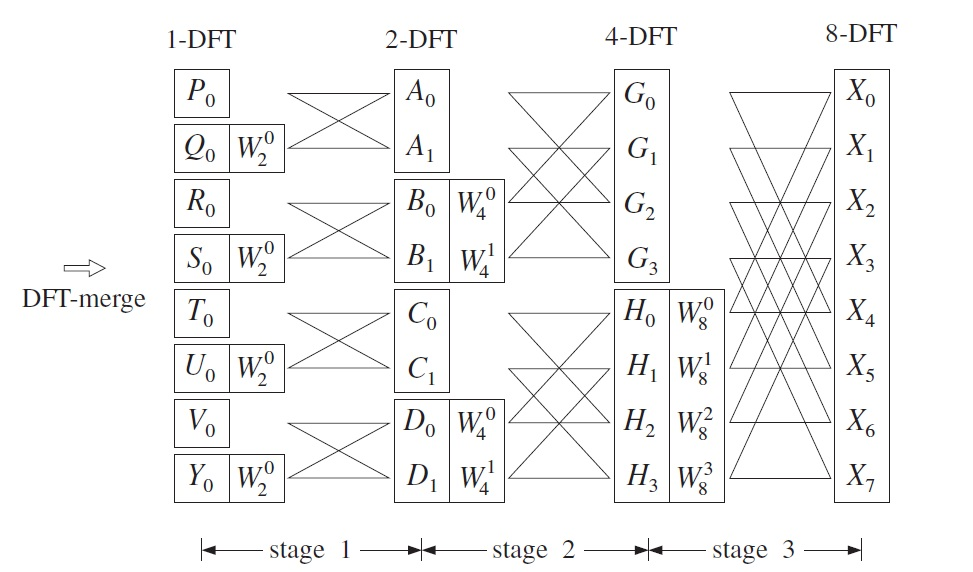
\includegraphics[width=\linewidth]{images/DFT_FFT_step2.jpg}
\end{center}

Note that the bit shuffling is also called bit reversal, because it has
the same effect as binary reversing the input.
\begin{center}
	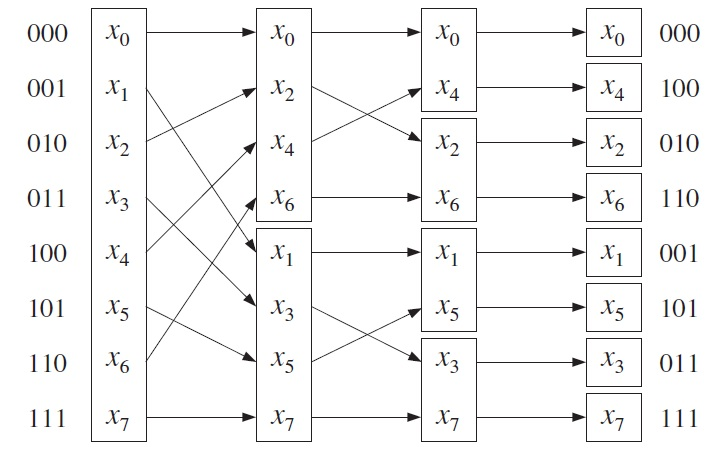
\includegraphics[width=0.8\linewidth]{images/DFT_FFT_shuffling.jpg}
\end{center}

\subsection{Fast Convolution\buchSeite{515-523}}
\subsubsection{Circular Convolution\buchSeite{515-520}}

\begin{equation*}
	\mathbf{y} = \mathbf{h} \ast \mathbf{x} \quad\Leftrightarrow\quad Y(\omega) = H(\omega) X(\omega)
\end{equation*}

This can also be achieved by using the DFT:
\begin{equation*}
	\tilde{\mathbf{y}} = \text{IDFT}(\DFT(\mathbf{h}) \cdot \DFT(\mathbf{x}))
\end{equation*}

But: the length $L_y$ of the convolution of a length $L$ and a length $M$
input is $L_y = L + M$. To prevent a \emph{circular convolution}, the
input vectors have to be zero-padded to a length of
\begin{equation*}
	N \geq L_y = L+M
\end{equation*}

\subsubsection{Overlap-Add and Overlap-Save Methods\buchSeite{520-523}}

\paragraph{Overlap-Add}
If the input signal $\mathbf{x}$ is of infinite length, no zero-padding
is possible. Then the input is divided into blocks
$\mathbf{x}_0, \mathbf{x}_1, \ldots$ which are processed separately.
The FFT length $N$ is of course $N \geq L+M$. As $M$ is saved and added
to the next result, no wraparound occurs.

\begin{center}
	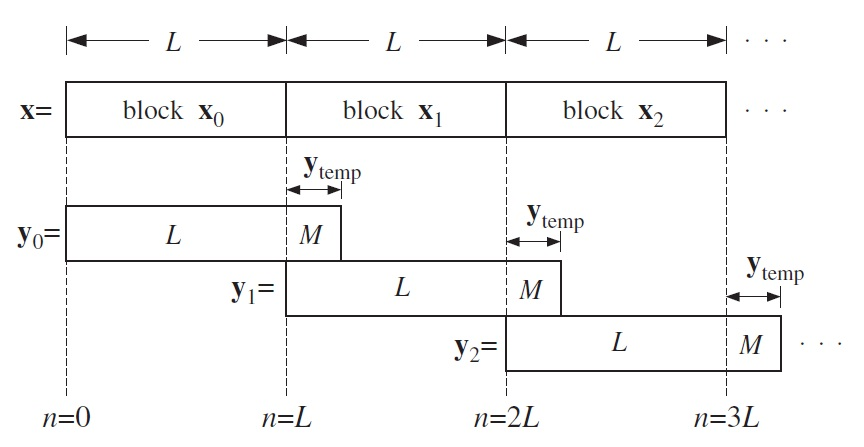
\includegraphics[width=0.9\linewidth]{images/DFT_FFT_overlapAdd.jpg}
\end{center}

The cost of the fast Overlap-Add method compared to the conventional, slow
method is
\begin{equation*}
	\frac{\text{fast}}{\text{slow}} = \frac{N (\log_2 N + 1)}{(M+1)(N-M)} \backsimeq \frac{\log_2 N}{M}
\end{equation*}

\paragraph{Overlap-Save}
Here, each block is of length $L=N$, but the blocks overlap by $M$. The output
blocks will have $M$ samples wrapped around, but as only the last $N-M$
samples are used, the $M$ wrapped around samples are not used at all.
(Though, the very first $M$ samples will be incorrect.)
\begin{center}
	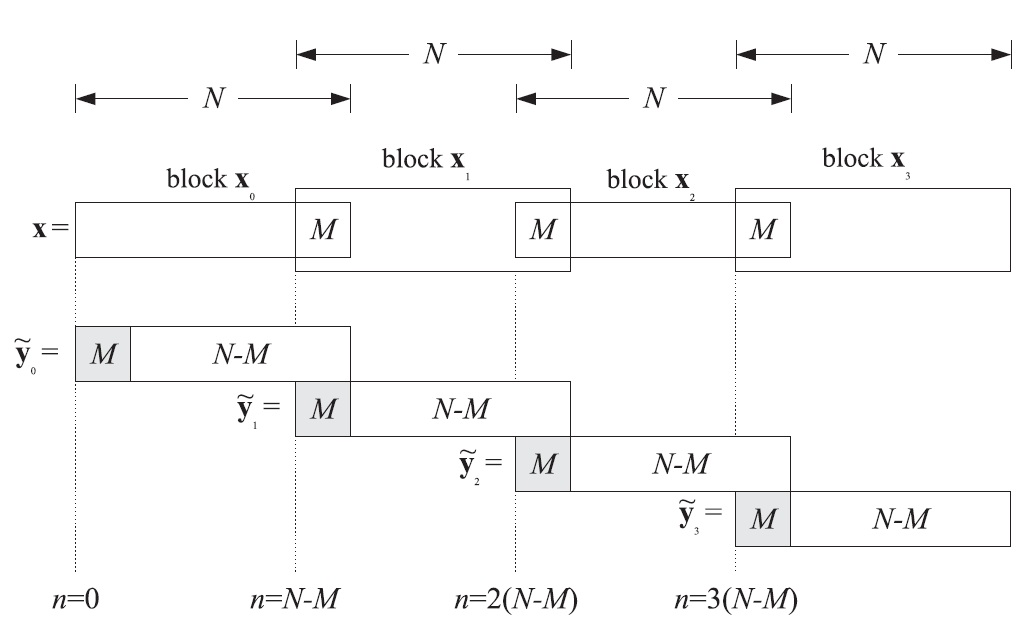
\includegraphics[width=0.9\linewidth]{images/DFT_FFT_overlapSave.jpg}
\end{center}
